\authoredSection{julius}{Kontexterkundung}
	Bei der Datenerhebung haben wir uns für eine Umfrage mittels Fragebogen entschieden, da die App in vielen verschiedenen Kontexten eingesetzt werden soll und wir möglichst viele Meinungen einfließen lassen wollten. 
	
	Für unser Konzept wollten wir wissen, welche Funktionen besonders beliebt sind und aus welchen Gründen die Teilnehmer Befürchtungen bei der Nutzung von Banking-Apps haben. Außerdem war es uns ein Anliegen nicht nur quantitative, sondern auch qualitative Daten zu erheben. Daher gab es Freitextfelder in denen die Teilnehmer Ideen, Kritik und allgemeine Bedenken in Bezug auf Banking-Apps äußern konnten. Dieses half uns die potentiellen Nutzer besser zu verstehen und Dinge aufzudecken, an die wir nicht gedacht hätten. An der Umfrage am Informatikum haben 92 Studenten teilgenommen
	
	Hier folgen nun die wichtigsten Ergebnisse. 

	Die Top 3 der nützlichsten Features sind der Bankautomatenfinder,  Filialenfinder und die Kartensperre. Der Bankautmatenfinder wurde von 93\% der Befragten als nützlich bewertet. Das sehr ähnliche Feature der Fialenfinder fanden 81\% nützlich und die Kartensperre wurde von 61\% als nützlich angesehen. Diese Ergebnisse zeigen, dass wir die Kernfeatures einer Banking-App nicht aus den Augen verlieren dürfen und dass ein optimierter Finder Potential hat.
	
	48\% der befragte Studenten hielten die Features „Depot-Verwaltung für Aktien“ und „Personalisierte Angebote der Bank“ als nicht nützlich.
	
	Eine mögliche Erklärung dafür ist, dass die Studenten bei diesen Themen einfach noch keine eigene Relevanz sehen. 
	
	Ein überraschendes Ergebnis der Umfrage war, dass nur 17\% der befragten Studenten eine Banking App nutzen. Für uns ist es natürlich interessant aus welchen Gründen Banking-Apps gemieden werden. Studenten gaben an „Apps sind zu unsicher“, „Apple, Microsoft und Co. würde Zugriff auf meine Daten haben“, „Unsicherheit der Datenübertragung“, „Bankgeschäfte sollte man in Ruhe bearbeiten und nicht hektisch to go“. In allen abgefragten Kategorien hatten mindestens über die Hälfte der Studenten Bedenken. Fast 80\% der befragten Studenten gaben an,  Angst vor den Missbrauch der Daten zu haben. Das zeigt, dass das Thema Sicherheit der eigenen Daten beim Banking eine Schlüsselrolle spielt und wir beim Konzept diesem Aspekt eine besondere Bedeutung zukommen lassen sollten.
	
\begin{figure}[p]
	\centering
	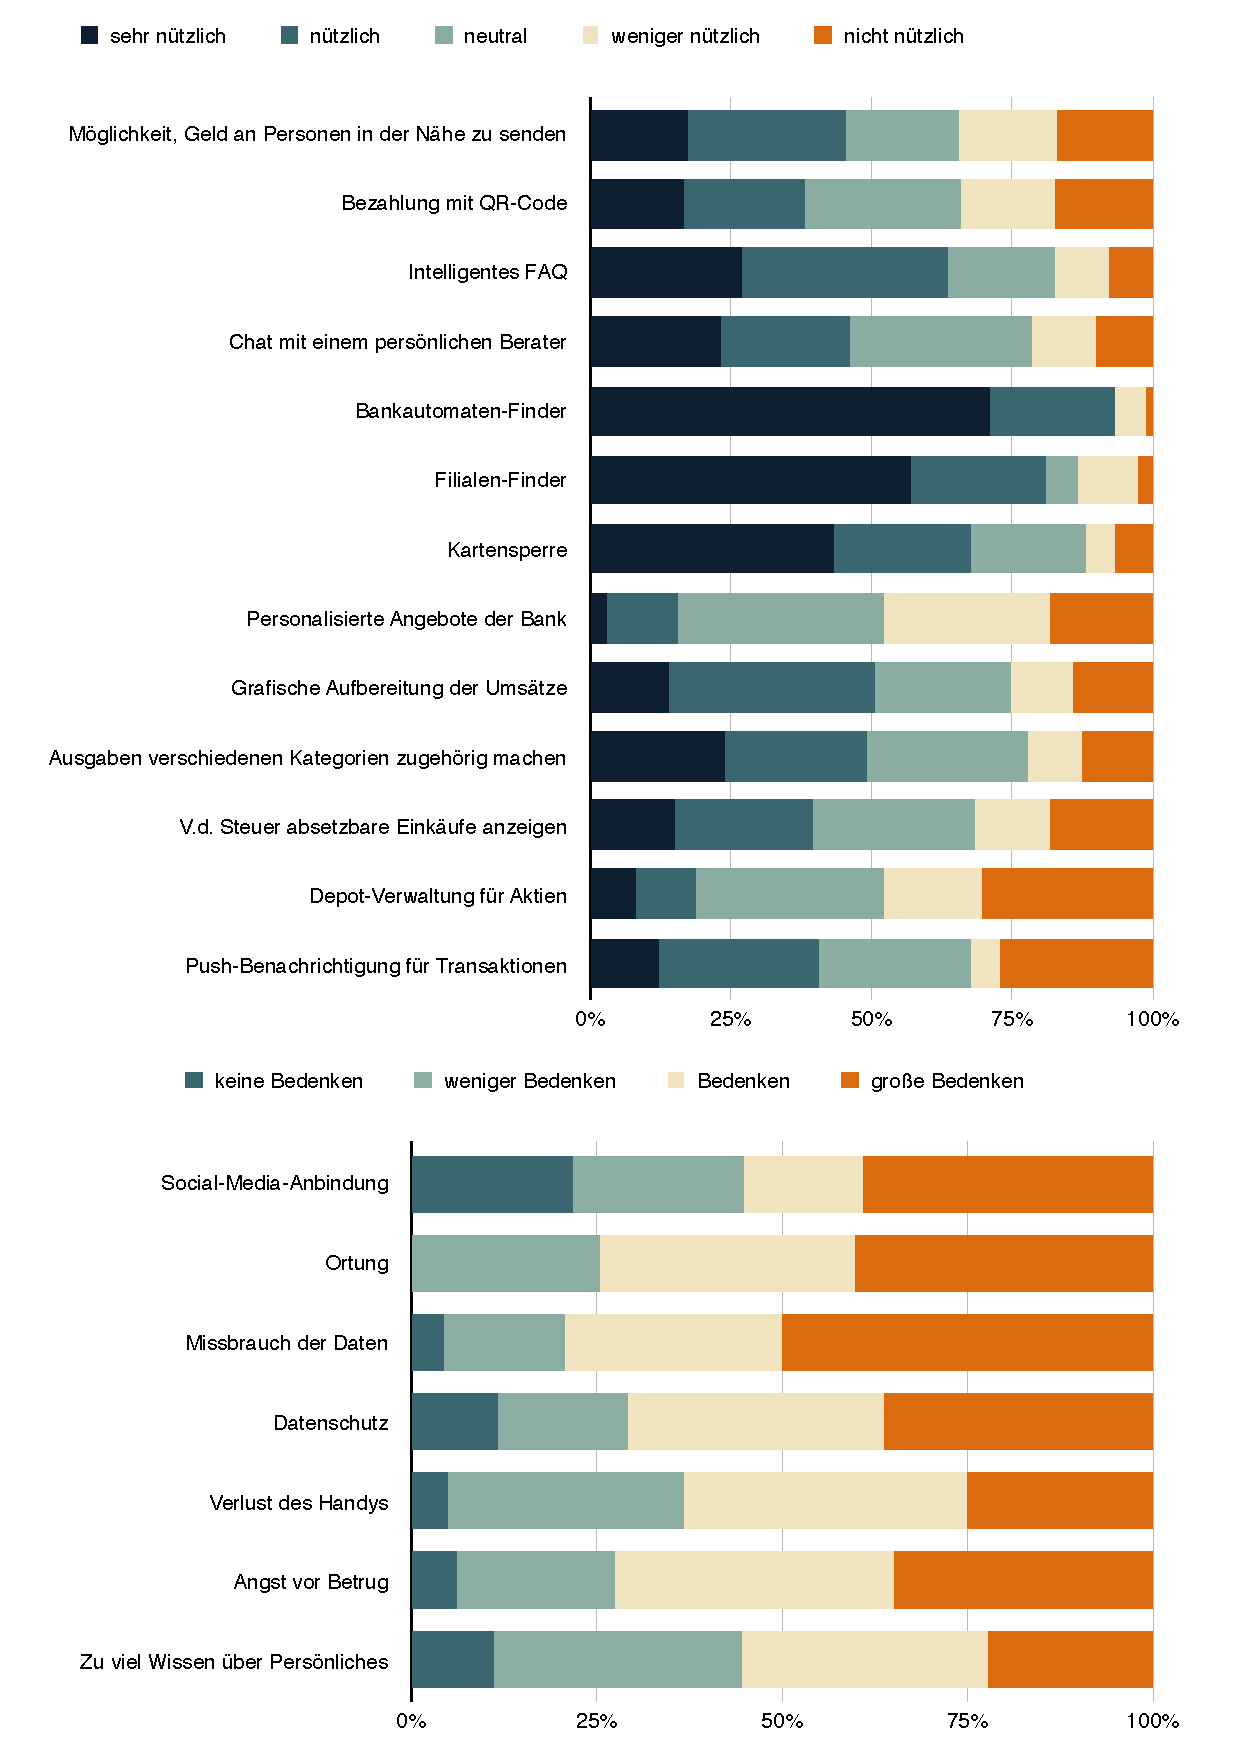
\includegraphics[scale=.69]{Pictures/Kontexterkundung}
	\caption{Ergebnisse der Kontexterkundung.}
\end{figure}